\documentclass[10pt,statementpaper]{memoir}

\setstocksize{9in}{6in}

\usepackage{tgpagella}
\usepackage{enumitem}
\usepackage{longtable}

\setlrmarginsandblock{0.5in}{0.5in}{*}
\setulmarginsandblock{0.6in}{0.6in}{*}
\checkandfixthelayout

\usepackage{etoolbox}
\patchcmd{\quote}{\rightmargin}{\leftmargin 1em \rightmargin}{}{}
\AtBeginEnvironment{quote}{\itshape}

\chapterstyle{southall}

\setlist[enumerate]{leftmargin=2em}
\setlist[itemize]{leftmargin=2em}

\usepackage{amssymb,amsmath}
\usepackage{ifxetex,ifluatex}
\usepackage{fixltx2e} % provides \textsubscript
\ifnum 0\ifxetex 1\fi\ifluatex 1\fi=0 % if pdftex
  \usepackage[$if(fontenc)$$fontenc$$else$T1$endif$]{fontenc}
  \usepackage[utf8]{inputenc}
\else % if luatex or xelatex
  \ifxetex
    \usepackage{mathspec}
  \else
    \usepackage{fontspec}
  \fi
  \defaultfontfeatures{Ligatures=TeX,Scale=MatchLowercase}
\fi
% use upquote if available, for straight quotes in verbatim environments
\IfFileExists{upquote.sty}{\usepackage{upquote}}{}
% use microtype if available
\IfFileExists{microtype.sty}{%
\usepackage[$for(microtypeoptions)$$microtypeoptions$$sep$,$endfor$]{microtype}
\UseMicrotypeSet[protrusion]{basicmath} % disable protrusion for tt fonts
}{}
\PassOptionsToPackage{hyphens}{url} % url is loaded by hyperref
\usepackage[unicode=true]{hyperref}
\hypersetup{
            pdfborder={0 0 0},
            breaklinks=true}
\urlstyle{same}  % don't use monospace font for urls

\usepackage{graphicx,grffile}
\makeatletter
\def\maxwidth{\ifdim\Gin@nat@width>\linewidth\linewidth\else\Gin@nat@width\fi}
\def\maxheight{\ifdim\Gin@nat@height>\textheight\textheight\else\Gin@nat@height\fi}
\makeatother
% Scale images if necessary, so that they will not overflow the page
% margins by default, and it is still possible to overwrite the defaults
% using explicit options in \includegraphics[width, height, ...]{}
\setkeys{Gin}{width=\maxwidth,height=\maxheight,keepaspectratio}

\setlength{\emergencystretch}{3em}  % prevent overfull lines
\providecommand{\tightlist}{%
  \setlength{\itemsep}{0pt}\setlength{\parskip}{0pt}}
\setcounter{secnumdepth}{$if(secnumdepth)$$secnumdepth$$else$5$endif$}

% set default figure placement to htbp
\makeatletter
\def\fps@figure{htbp}
\makeatother

\begin{document}

\pagestyle{empty}

{\begingroup
  \raggedleft
  \vspace*{\baselineskip}

  {\Huge\itshape How to Teach Programming \\ (And Other Things)}\\[\baselineskip]

  {\large\itshape
    what everyone in tech ought to know\\ about teaching and learning
  }\\[0.2\textheight]

  {\large Edited by Greg Wilson}\par

  \vfill

  {\large Copyright {\copyright} 2017}

  \vspace*{\baselineskip}

  {\small
    Licensed under the Creative Commons - Attribution license (CC-BY-3.0).
    \\
    See \texttt{https://github.com/gvwilson/thirdbit} for the source,\\
    and \texttt{http://third-bit.com/teaching/} for the online version.
  }

  \vspace*{4\baselineskip}

  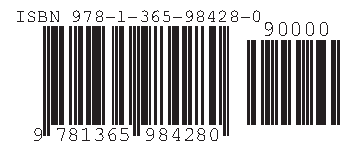
\includegraphics{isbn-barcode.pdf}

\endgroup}

\newpage

\pagestyle{empty}

~

\newpage

\addtocontents{toc}{\protect\thispagestyle{empty}}
\tableofcontents

\newpage

\pagestyle{empty}

~

\newpage

\pagestyle{plain}
\pagenumbering{arabic}

$body$

\end{document}
